%==============================================================
%  EE201 -- Circuit Theory I
%  Lecture 9 : Trees, Cutsets and Fundamental Loops -- slides
%  M. Mert Ankaralı, METU EEE
%
%  Compile:  ./build.sh      (or: pdflatex EE201_Lecture_9_slides.tex, twice)
%  Same colour code as the handout:
%      charge = purple, current = blue, voltage = orange, power = green
%==============================================================
\documentclass[11pt,aspectratio=169]{beamer}

\usepackage[T1]{fontenc}
\usepackage[utf8]{inputenc}
\usepackage[english]{babel}
\usepackage{lmodern}
\usepackage{amsmath,amssymb}
\usepackage{booktabs}
\usepackage{array}
\usepackage{colortbl}
\usepackage{tikz}
\usepackage[american,siunitx]{circuitikz}
\usetikzlibrary{matrix,arrows.meta,positioning,calc,decorations.pathreplacing,decorations.pathmorphing,decorations.markings}
\usetikzlibrary{overlay-beamer-styles}

%-------------------- plain METU-flavoured theme --------------
\usetheme{default}
\usecolortheme{default}
\useinnertheme{rectangles}
\setbeamertemplate{navigation symbols}{}
\setbeamertemplate{itemize items}[square]
\setbeamerfont{frametitle}{size=\large,series=\bfseries}
\setbeamerfont{title}{size=\LARGE,series=\bfseries}

\definecolor{metured}{RGB}{155,27,48}
\definecolor{metugray}{RGB}{88,89,91}
\definecolor{metulight}{RGB}{243,240,241}
\definecolor{ccur}{RGB}{0,102,170}
\definecolor{cvolt}{RGB}{214,120,0}
\definecolor{cpow}{RGB}{23,128,74}
\definecolor{ccharge}{RGB}{124,60,160}
\definecolor{cflux}{RGB}{0,138,138}
\definecolor{copper}{RGB}{184,98,30}

\setbeamercolor{structure}{fg=metured}
\setbeamercolor{frametitle}{fg=metured,bg=}
\setbeamercolor{title}{fg=metured}
\setbeamercolor{normal text}{fg=black!88}
\setbeamercolor{block title}{fg=white,bg=metured}
\setbeamercolor{block body}{bg=metulight}
\setbeamercolor{alerted text}{fg=metured}

\setbeamertemplate{frametitle}{%
  \vspace{0.55em}%
  \usebeamerfont{frametitle}\usebeamercolor[fg]{frametitle}\insertframetitle\par
  \vspace{-0.2em}{\color{metured}\rule{\textwidth}{1pt}}\par\vspace{-0.2em}}

\setbeamertemplate{footline}{%
  \hbox{\begin{beamercolorbox}[wd=\paperwidth,ht=2.4ex,dp=1.4ex,leftskip=1.2em,rightskip=1.2em]{}%
  \tiny\color{metugray}\coursecode\ \textbar\ Lecture 9: Trees, Cutsets and Fundamental Loops
  \hfill \insertframenumber/\inserttotalframenumber
  \end{beamercolorbox}}}

%-------------------- macros ----------------------------------
\newcommand{\coursecode}{EE201}
\newcommand{\term}{Fall 2026--2027}
\newcommand{\Icol}[1]{\textcolor{ccur}{#1}}
\newcommand{\Vcol}[1]{\textcolor{cvolt}{#1}}
\newcommand{\Pcol}[1]{\textcolor{cpow}{#1}}
\newcommand{\Qcol}[1]{\textcolor{ccharge}{#1}}
\newcommand{\Fcol}[1]{\textcolor{cflux}{#1}}
\newcommand{\uni}[1]{\,\mathrm{#1}}
\newcommand{\A}{\uni{A}} \newcommand{\V}{\uni{V}}
\newcommand{\W}{\uni{W}} \newcommand{\J}{\uni{J}}
\newcommand{\Cb}{\uni{C}} \newcommand{\s}{\uni{s}}
\newcommand{\Wb}{\uni{Wb}} \newcommand{\Hy}{\uni{H}}
\newcommand{\Sie}{\uni{S}}


\ctikzset{bipoles/length=0.9cm, label/align=straight,
          bipoles/generic/height=0.28, bipoles/generic/width=0.62}
\tikzset{
  iar/.style={-{Stealth[length=2.2mm]}, ccur, thick},
  glab/.style={font=\footnotesize, text=metured},
  ttl/.style={font=\scriptsize\bfseries, text=metugray},
  capn/.style={font=\scriptsize, text=metugray, align=center},
  pol/.style={font=\small, text=cvolt},
  nlab/.style={circle, draw=metured, text=metured, font=\scriptsize, inner sep=0.7pt},
  blab/.style={font=\footnotesize, text=black!80},
  gbr/.style={black!75, thick, postaction={decorate, decoration={markings,
      mark=at position 0.56 with {\arrow{Stealth[length=2.5mm]}}}}},
  hal/.style={draw=cpow!60, line width=6pt, opacity=0.35, line cap=round, line join=round},
  halo/.style={circle, fill=metured!16, minimum size=0.95cm},
  elem/.style={draw=metugray, thick, fill=metulight},
  bigarr/.style={-{Stealth[length=3mm]}, very thick, metugray},
}

\newcommand{\nd}[1]{\tikz[baseline=(c.base)]\node[nlab](c){#1};}
\newcommand{\brarr}[4]{%
  \draw[iar] ($(#1)!0.34!(#2)!0.34cm!#3:(#2)$) -- ($(#1)!0.66!(#2)!0.34cm!#3:(#2)$);
  \node[blab] at ($(#1)!0.5!(#2)!0.66cm!#3:(#2)$) {#4};}
\newcommand{\gbranch}[4]{%
  \draw[gbr] (#1) -- (#2);
  \node[blab] at ($(#1)!0.5!(#2)!0.28cm!#3:(#2)$) {#4};}
%  An incidence matrix with node labels on the left and branch numbers on top.
%  #1 name, #2 number of columns, #3 node labels, #4 rows (entries separated by \&),
%  #5 extra TikZ code drawn on top (may refer to the cells #1-i-j)
\newcommand{\incmat}[5]{%
  \begin{tikzpicture}[baseline={([yshift=-0.6ex]#1.center)}]
    \matrix (#1) [matrix of math nodes, ampersand replacement=\&,
                  left delimiter={[}, right delimiter={]}, inner sep=1pt,
                  column sep=0.45em,
                  nodes={text width=1.35em, align=right, minimum height=1.25em,
                         inner sep=1pt}] {#4};
    \foreach \j in {1,...,#2}
      \node[font=\scriptsize, text=metugray, anchor=south east, inner sep=1pt]
        at ([yshift=2pt]#1-1-\j.north east) {\j};
    \foreach \lab [count=\i] in {#3}
      \node[nlab, left=11pt] at (#1.west |- #1-\i-1) {\lab};
    #5
  \end{tikzpicture}}
\newcommand{\xfmr}[2]{%
  \begin{scope}[xshift=#1 cm]
    \ctikzset{bipoles/length=1.35cm}
    \draw (0,0) to[L] (0,#2);
    \draw (1.6,#2) to[L] (1.6,0);
    \draw[line width=1.1pt, metugray] (0.72,-0.05) -- (0.72,#2+0.05);
    \draw[line width=1.1pt, metugray] (0.88,-0.05) -- (0.88,#2+0.05);
    \fill (0.36,#2-0.2) circle (2.1pt);
    \fill (1.24,#2-0.2) circle (2.1pt);
  \end{scope}}
%  Same, with explicit column labels: #1 name, #2 column labels, #3 row labels,
%  #4 rows, #5 extra TikZ code
\newcommand{\incmatc}[5]{%
  \begin{tikzpicture}[baseline={([yshift=-0.6ex]#1.center)}]
    \matrix (#1) [matrix of math nodes, ampersand replacement=\&,
                  left delimiter={[}, right delimiter={]}, inner sep=1pt,
                  column sep=0.45em,
                  nodes={text width=1.35em, align=right, minimum height=1.25em,
                         inner sep=1pt}] {#4};
    \foreach \lab [count=\j] in {#2}
      \node[font=\scriptsize, text=metugray, anchor=south east, inner sep=1pt]
        at ([yshift=2pt]#1-1-\j.north east) {\lab};
    \foreach \lab [count=\i] in {#3}
      \node[nlab, left=11pt] at (#1.west |- #1-\i-1) {\lab};
    #5
  \end{tikzpicture}}
\newcommand{\bridgecoords}{%
  \coordinate (n1) at (0,1.7);  \coordinate (n2) at (-1.5,0);
  \coordinate (n3) at (1.5,0);  \coordinate (n4) at (0,-1.7);}
\newcommand{\bridgenodes}{%
  \foreach \k/\pos in {1/above, 2/left, 3/right, 4/below}
    {\fill[metured] (n\k) circle (2.2pt); \node[nlab, \pos=3pt] at (n\k) {\k};}}
\newcommand{\bridgecircuit}{%
  \draw (n1) to[generic] (n2);  \draw (n1) to[generic] (n3);
  \draw (n3) to[generic] (n2);  \draw (n2) to[generic] (n4);
  \draw (n3) to[generic] (n4);
  \coordinate (s6) at (-2.6,-1.7); \coordinate (e6) at (-2.6,1.7);
  \draw (n4) -- (s6) to[generic] (e6) -- (n1);}
\newcommand{\bridgegraph}{%
  \gbranch{n1}{n2}{-90}{1}  \gbranch{n1}{n3}{90}{2}  \gbranch{n3}{n2}{-90}{3}
  \gbranch{n2}{n4}{-90}{4}  \gbranch{n3}{n4}{90}{5}
  \draw[gbr] (n4) to[out=180, in=180, looseness=2.3] (n1);
  \node[blab] at (-2.55,0) {6};
  \bridgenodes}
%  A graph branch from #1 to #2 with its branch voltage: + near the tail, - near the head,
%  v_#4 in the middle; #3 = auto=left or auto=right picks the side
\newcommand{\gvbranch}[4]{%
  \draw[gbr] (#1) --
    node[pos=0.27, #3, pol, inner sep=1pt] {$+$}
    node[pos=0.5, #3, font=\small, text=cvolt, inner sep=2.5pt] {$v_{#4}$}
    node[pos=0.73, #3, pol, inner sep=1pt] {$-$} (#2);}
\newcommand{\bridgevgraph}{%
  \gvbranch{n1}{n2}{auto=right}{1}  \gvbranch{n1}{n3}{auto=left}{2}
  \gvbranch{n3}{n2}{auto=right}{3}  \gvbranch{n2}{n4}{auto=right}{4}
  \gvbranch{n3}{n4}{auto=left}{5}
  \draw[gbr] (n4) to[out=180, in=180, looseness=2.3]
    node[pos=0.22, left, pol, inner sep=2pt] {$+$}
    node[pos=0.5, left, font=\small, text=cvolt] {$v_6$}
    node[pos=0.78, left, pol, inner sep=2pt] {$-$} (n1);
  \bridgenodes}
%  One branch, for the definition: + at the tail, - at the head, current along the arrow
\newcommand{\onebranch}{%
  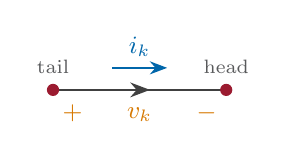
\begin{tikzpicture}[baseline=-0.6ex]
    \coordinate (p) at (0,0); \coordinate (q) at (2.2,0);
    \draw[gbr] (p) -- (q);
    \fill[metured] (p) circle (2.2pt); \fill[metured] (q) circle (2.2pt);
    \node[pol] at (0.25,-0.3) {$+$}; \node[pol] at (1.95,-0.3) {$-$};
    \node[font=\small, text=cvolt] at (1.1,-0.32) {$v_k$};
    \draw[iar] (0.75,0.28) -- (1.45,0.28); \node[font=\small, text=ccur] at (1.1,0.55) {$i_k$};
    \node[font=\scriptsize, text=metugray] at (0,0.3) {tail};
    \node[font=\scriptsize, text=metugray] at (2.2,0.3) {head};
  \end{tikzpicture}}
\newcommand{\U}[2]{\uncover<#1->{#2}}
\providecommand{\ohm}{\,\Omega}

\hypersetup{colorlinks=true,allcolors=metured}

\title{Lecture 9: Trees, Cutsets\\ and Fundamental Loops}
\subtitle{EE201 -- Circuit Theory I}
\author{M. Mert Ankaralı}
\institute{\small Department of Electrical and Electronics Engineering\\
           Middle East Technical University}
\date{}

%==============================================================
%-------------------- Lecture 8 additions ---------------------
\tikzset{mlabst/.style={draw=ccur, text=ccur, fill=white, rounded corners=1.5pt,
                        inner sep=1.2pt, font=\scriptsize\bfseries}}
%  A boxed mesh number, for the text
\newcommand{\mlab}[1]{\tikz[baseline=(c.base)]\node[mlabst](c){#1};}
%  A clockwise mesh arrow at (#2,#3) with mesh number #4; optional radius #1
\newcommand{\meshcw}[4][0.32]{%
  \draw[ccur, thick, -{Stealth[length=2mm]}] ($(#2,#3)+(150:#1)$)
    arc[start angle=150, end angle=-150, radius=#1];
  \node[mlabst] at (#2,#3) {#4};}
%  The three inner meshes of the bridge graph (after \bridgecoords)
\newcommand{\bridgemeshes}{%
  \meshcw[0.3]{0}{0.82}{1} \meshcw[0.3]{0}{-0.78}{2} \meshcw[0.24]{-1.55}{0.66}{3}}
\newcommand{\fillmeshA}[1][]{\fill[ccur!14, #1] (n1) -- (n2) -- (n3) -- cycle;}
\newcommand{\fillmeshB}[1][]{\fill[ccur!14, #1] (n2) -- (n3) -- (n4) -- cycle;}
\newcommand{\fillmeshC}[1][]{\fill[ccur!14, #1] (n4) to[out=180, in=180, looseness=2.3] (n1) -- (n2) -- cycle;}
%  The bridge graph drawn as a square: both diagonals cross
%  Separable / nonseparable pictures: before and after removing one node.
%  Removed node: open grey circle; removed branches: dashed grey.
\tikzset{gone/.style={gray!55, thick, dash pattern=on 2.5pt off 2pt},
  gonenode/.style={gray!70, thick, fill=white},
  gonelab/.style={nlab, draw=gray!70, text=gray!70}}
\newcommand{\twotricoords}{%
  \coordinate (c) at (1.6,0.8);
  \coordinate (a1) at (0,1.6); \coordinate (a2) at (0,0);
  \coordinate (b1) at (3.2,1.6); \coordinate (b2) at (3.2,0);}
\newcommand{\twotri}{%
  \twotricoords
  \draw[black!75, thick] (c) -- (a1) -- (a2) -- cycle;
  \draw[black!75, thick] (c) -- (b1) -- (b2) -- cycle;
  \foreach \p in {a1,a2,b1,b2,c} \fill[metured] (\p) circle (2.2pt);}
\newcommand{\twotricut}{%
  \twotricoords
  \draw[gone] (a1) -- (c) -- (a2);  \draw[gone] (b1) -- (c) -- (b2);
  \draw[cvolt, very thick] (a1) -- (a2);  \draw[ccur, very thick] (b1) -- (b2);
  \foreach \p in {a1,a2,b1,b2} \fill[metured] (\p) circle (2.2pt);
  \draw[gonenode] (c) circle (2.6pt);}
%  N with node 2 removed: branches 1, 3, 4 go; 2, 5, 6 stay (one piece)
\newcommand{\bridgecut}{%
  \bridgecoords
  \draw[gone] (n1) -- (n2);  \draw[gone] (n3) -- (n2);  \draw[gone] (n2) -- (n4);
  \begin{scope}[gbr/.append style={ccur, very thick}]
    \gbranch{n1}{n3}{90}{2}  \gbranch{n3}{n4}{90}{5}
    \draw[gbr] (n4) to[out=180, in=180, looseness=2.3] (n1);
  \end{scope}
  \node[blab] at (-2.55,0) {6};
  \foreach \k/\pos in {1/above, 3/right, 4/below}
    {\fill[metured] (n\k) circle (2.2pt); \node[nlab, \pos=3pt] at (n\k) {\k};}
  \draw[gonenode] (n2) circle (2.6pt);
  \node[gonelab, left=3pt] at (n2) {2};}
%  Separable vs nonseparable, before and after removing a node. #1, #3: extra options
%  for the two "after" pictures; #2, #4: for the removed parts drawn in them
%  (overlay styles on slides, empty in the notes)
\newcommand{\nsepfigure}[4]{%
  \begin{tikzpicture}[scale=0.8]
    \begin{scope}
      \twotri
      \node[ttl] at (1.6,-1.2) {separable};
    \end{scope}
    \begin{scope}[#1]
      \draw[bigarr] (3.6,0.8) -- (4.4,0.8);
      \node[capn] at (4.0,1.35) {remove\\ centre};
      \begin{scope}[xshift=4.8cm, gone/.append style={#2}, gonenode/.append style={#2}]
        \twotricut
      \end{scope}
      \node[ttl] at (6.4,-1.2) {\textcolor{cvolt}{two} \textcolor{ccur}{pieces}};
    \end{scope}
    \draw[metugray!50] (8.7,-1.4) -- (8.7,2.3);
    \begin{scope}[xshift=11.0cm, yshift=0.8cm, scale=0.75, transform shape]
      \bridgecoords \bridgegraph
    \end{scope}
    \node[ttl] at (10.6,-1.2) {nonseparable (bridge)};
    \begin{scope}[#3]
      \draw[bigarr] (12.55,0.8) -- (13.45,0.8);
      \node[capn] at (13.0,1.35) {remove\\ node 2};
      \begin{scope}[xshift=15.9cm, yshift=0.8cm, scale=0.75, transform shape,
                    gone/.append style={#4}, gonenode/.append style={#4},
                    gonelab/.append style={#4}]
        \bridgecut
      \end{scope}
      \node[ttl] at (15.5,-1.2) {\textcolor{ccur}{still one piece}};
    \end{scope}
  \end{tikzpicture}}
\newcommand{\squarekfour}{%
  \coordinate (s1) at (0,2); \coordinate (s3) at (2,2);
  \coordinate (s4) at (2,0); \coordinate (s2) at (0,0);
  \foreach \u/\v/\k/\lp in {s1/s2/1/left, s1/s3/2/above, s2/s4/4/below, s3/s4/5/right}
    \draw[black!75, thick] (\u) -- (\v) node[midway, \lp, blab] {\k};
  \draw[black!75, thick] (s3) -- (s2) node[pos=0.25, above left, blab, inner sep=1pt] {3};
  \draw[black!75, thick] (s4) -- (s1) node[pos=0.25, above right, blab, inner sep=1pt] {6};
  \foreach \k/\pos in {1/above left, 2/below left, 3/above right, 4/below right}
    {\fill[metured] (s\k) circle (2.2pt); \node[nlab, \pos=1pt] at (s\k) {\k};}}
%  The circuit of the Tellegen example (10 V, 2, 4, 12 ohm), with current references
%  A hop (bump): the wire passes over another one without touching it.
%  \hopseg{P}{X}{Q}: from P to Q, jumping at the crossing point X
\newcommand{\hopr}{0.22cm}
\newcommand{\hopseg}[3]{%
  ($(#2)!\hopr!(#1)$) to[bend left=90, looseness=1.55] ($(#2)!\hopr!(#3)$)}
%  The square drawing of the bridge graph, branch 6 hopping over branch 3
\newcommand{\squarehop}{%
  \coordinate (s1) at (0,2); \coordinate (s3) at (2,2);
  \coordinate (s4) at (2,0); \coordinate (s2) at (0,0);
  \coordinate (sx) at (1,1);
  \foreach \u/\v/\k/\lp in {s1/s2/1/left, s1/s3/2/above, s2/s4/4/below, s3/s4/5/right}
    \draw[black!75, thick] (\u) -- (\v) node[midway, \lp, blab] {\k};
  \draw[black!75, thick] (s3) -- (s2) node[pos=0.25, above left, blab, inner sep=1pt] {3};
  \draw[copper, very thick] (s4) -- \hopseg{s4}{sx}{s1} -- (s1);
  \node[blab, text=copper] at (1.62,0.62) {6};
  \foreach \k/\pos in {1/above left, 2/below left, 3/above right, 4/below right}
    {\fill[metured] (s\k) circle (2.2pt); \node[nlab, \pos=1pt] at (s\k) {\k};}}
%  The nonplanar hexagon graph with as few hops as possible: one diagonal goes around
%  the outside, and one hop is still left
\newcommand{\hexhop}{%
  \foreach \a/\n in {0/a,60/b,120/c,180/d,240/e,300/f} \coordinate (\n) at (\a:1.15);
  \draw[black!75, thick] (a) -- (b) -- (c) -- (d) -- (e) -- (f) -- cycle;
  \draw[black!75, thick] (a) -- (d);
  \draw[black!75, thick] (b) .. controls (3.1,2.2) and (0.6,-3.3) .. (e);
  \draw[copper, very thick] (c) -- \hopseg{c}{0,0}{f} -- (f);
  \foreach \n in {a,b,c,d,e,f} \fill[metured] (\n) circle (2.2pt);}
%  The same graph in 3D: hexagon on a board, diagonals lifted to different heights.
%  #1: the x, y, z unit vectors of the view
\newcommand{\hexthreeD}[1]{%
  \begin{scope}[#1]
    \fill[metulight] (-1.55,-1.55,0) -- (1.55,-1.55,0) -- (1.55,1.55,0) -- (-1.55,1.55,0) -- cycle;
    \draw[gray!45] (-1.55,-1.55,0) -- (1.55,-1.55,0) -- (1.55,1.55,0) -- (-1.55,1.55,0) -- cycle;
    \foreach \a in {0,60,...,300}
      \draw[black!75, thick] ({1.15*cos(\a)},{1.15*sin(\a)},0) -- ({1.15*cos(\a+60)},{1.15*sin(\a+60)},0);
    \draw[black!75, thick] ({1.15*cos(120)},{1.15*sin(120)},0) -- ({-1.15*cos(120)},{-1.15*sin(120)},0);
    \foreach \a/\h in {0/0.6, 60/1.15}
      \draw[copper, very thick] plot[domain=0:1, samples=31, variable=\t]
        ({1.15*cos(\a)*(1-2*\t)},{1.15*sin(\a)*(1-2*\t)},{\h*sin(180*\t)});
    \foreach \a in {0,60,...,300} \fill[metured] ({1.15*cos(\a)},{1.15*sin(\a)},0) circle (2.2pt);
  \end{scope}}
\tikzset{
  view top/.style={x={(1cm,0cm)}, y={(0cm,1cm)}, z={(0cm,0cm)}},
  view oblique/.style={x={(0.9cm,-0.32cm)}, y={(0.9cm,0.32cm)}, z={(0cm,0.95cm)}},
  view side/.style={x={(1cm,0cm)}, y={(0.22cm,0.1cm)}, z={(0cm,0.95cm)}},
}
\newcommand{\tcircuit}[1]{%
\begin{tikzpicture}[scale=#1]
  \draw (0,0) to[american voltage source, invert] (0,2.2);
  \node[font=\small, left] at (-0.45,1.1) {$10\V$};
  \draw (0,2.2) to[R] (2.6,2.2);
  \node[font=\small] at (1.3,2.62) {$2\ohm$};
  \draw (2.6,2.2) -- (4.4,2.2);
  \draw (2.6,2.2) to[R] (2.6,0);
  \node[font=\small, right] at (2.85,1.75) {$4\ohm$};
  \draw (4.4,2.2) to[R] (4.4,0);
  \node[font=\small, right] at (4.65,1.1) {$12\ohm$};
  \draw (4.4,0) -- (0,0);
  \draw[iar] (0.55,0.7) -- (0.55,1.5);  \node[font=\small, text=ccur] at (0.85,1.1) {$i_1$};
  \draw[iar] (0.85,1.8) -- (1.75,1.8);  \node[font=\small, text=ccur] at (1.3,1.5) {$i_2$};
  \draw[iar] (2.25,1.45) -- (2.25,0.75); \node[font=\small, text=ccur] at (1.95,1.1) {$i_3$};
  \draw[iar] (4.05,1.45) -- (4.05,0.75); \node[font=\small, text=ccur] at (3.75,1.1) {$i_4$};
  \foreach \x/\y/\k/\pos in {0/2.2/1/above left, 2.6/2.2/2/above, 1.3/0/3/below}
    {\fill[metured] (\x,\y) circle (2.2pt); \node[nlab, \pos=2pt] at (\x,\y) {\k};}
  \meshcw[0.28]{1.3}{0.65}{1}
  \meshcw[0.28]{3.3}{0.6}{2}
\end{tikzpicture}}
%  A mesh matrix: like \incmat, with mesh numbers as row labels
\newcommand{\incmatm}[4]{%
  \begin{tikzpicture}[baseline={([yshift=-0.6ex]#1.center)}]
    \matrix (#1) [matrix of math nodes, ampersand replacement=\&,
                  left delimiter={[}, right delimiter={]}, inner sep=1pt,
                  column sep=0.45em,
                  nodes={text width=1.35em, align=right, minimum height=1.25em,
                         inner sep=1pt}] {#4};
    \foreach \j in {1,...,#2}
      \node[font=\scriptsize, text=metugray, anchor=south east, inner sep=1pt]
        at ([yshift=2pt]#1-1-\j.north east) {\j};
    \foreach \lab [count=\i] in {#3}
      \node[mlabst, left=11pt] at (#1.west |- #1-\i-1) {\lab};
  \end{tikzpicture}}
%  Slides only: the mesh matrix of N, row k shown from overlay k+1 on
\newcommand{\incmatmv}[4]{%
  \begin{tikzpicture}[baseline={([yshift=-0.6ex]#1.center)}]
    \matrix (#1) [matrix of math nodes, ampersand replacement=\&,
                  left delimiter={[}, right delimiter={]}, inner sep=1pt,
                  column sep=0.45em,
                  nodes={text width=1.35em, align=right, minimum height=1.25em,
                         inner sep=1pt},
                  row 1/.style={nodes={visible on=<2->}},
                  row 2/.style={nodes={visible on=<3->}},
                  row 3/.style={nodes={visible on=<4->}}] {#4};
    \foreach \j in {1,...,#2}
      \node[font=\scriptsize, text=metugray, anchor=south east, inner sep=1pt]
        at ([yshift=2pt]#1-1-\j.north east) {\j};
    \foreach \lab [count=\i] in {#3}
      \node[mlabst, left=11pt] at (#1.west |- #1-\i-1) {\lab};
  \end{tikzpicture}}

%==============================================================
%-------------------- Lecture 9 additions ---------------------
\definecolor{ctree}{RGB}{23,128,74}      % tree branches -- green
\tikzset{
  treebr/.style={gbr, ctree, line width=2.1pt},
  cotreebr/.style={gbr},
  hlbr/.style={gbr, cvolt, line width=2.1pt},
  faintbr/.style={black!22, thick},
  plainbr/.style={black!75, thick},
  surf/.style={cvolt, thick, dash pattern=on 3pt off 2pt},
}
%  A straight branch from #1 to #2, number #4 on side #3, drawn with style #5
\newcommand{\sbranch}[5]{%
  \draw[#5] (#1) -- (#2);
  \node[blab] at ($(#1)!0.5!(#2)!0.28cm!#3:(#2)$) {#4};}
%  The bridge graph with a style for each of its six branches
\newcommand{\bridgesub}[6]{%
  \sbranch{n1}{n2}{-90}{1}{#1}  \sbranch{n1}{n3}{90}{2}{#2}  \sbranch{n3}{n2}{-90}{3}{#3}
  \sbranch{n2}{n4}{-90}{4}{#4}  \sbranch{n3}{n4}{90}{5}{#5}
  \draw[#6] (n4) to[out=180, in=180, looseness=2.3] (n1);
  \node[blab] at (-2.55,0) {6};
  \bridgenodes}
%  The graph G of this lecture: 4 nodes, 6 branches (branch 5 curved, parallel to 4)
\newcommand{\tgcoords}{%
  \coordinate (g1) at (-1,1.73); \coordinate (g2) at (1,1.73);
  \coordinate (g3) at (-2,0);    \coordinate (g4) at (0,0);}
\newcommand{\tgnodes}{%
  \foreach \k/\pos in {1/above, 2/above, 3/below left, 4/below}
    {\fill[metured] (g\k) circle (2.2pt); \node[nlab, \pos=2pt] at (g\k) {\k};}}
%  G with a style for each branch (#1 ... #6 = branches 1 ... 6)
\newcommand{\tgraph}[6]{%
  \sbranch{g2}{g1}{-90}{1}{#1}  \sbranch{g1}{g3}{-90}{2}{#2}  \sbranch{g1}{g4}{90}{3}{#3}
  \sbranch{g2}{g4}{90}{4}{#4}
  \draw[#5] (g2) to[out=-10, in=0, looseness=1.6] node[blab, pos=0.5, right=1pt] {5} (g4);
  \sbranch{g3}{g4}{-90}{6}{#6}
  \tgnodes}
%  G with its tree {1,3,6} in green
\newcommand{\tgtree}{\tgraph{treebr}{cotreebr}{treebr}{cotreebr}{cotreebr}{treebr}}
%  The figure-eight graph of the cutset example (no arrows)
\newcommand{\eightcoords}{%
  \coordinate (eL) at (-3.0,0); \coordinate (eT) at (-1.7,1.05); \coordinate (eM) at (0,0);
  \coordinate (eP) at (1.6,1.05); \coordinate (eR) at (3.0,0);}
\newcommand{\eightgraph}{%
  \draw[plainbr] (eL) to[bend left=25] node[blab, above left=-1pt] {2} (eT);
  \draw[plainbr] (eT) to[bend left=12] node[blab, above=1pt] {3} (eM);
  \draw[plainbr] (eL) to[bend right=30] node[blab, below=1pt] {1} (eM);
  \draw[plainbr] (eM) to[bend left=35] node[blab, above left=-1pt] {4} (eP);
  \draw[plainbr] (eM) to[bend right=15] node[blab, below right=-2pt] {5} (eP);
  \draw[plainbr] (eP) to[bend left=25] node[blab, above right=-1pt] {7} (eR);
  \draw[plainbr] (eM) to[bend right=30] node[blab, below=1pt] {6} (eR);
  \foreach \p in {eL,eT,eM,eP,eR} \fill[metured] (\p) circle (2.2pt);}
%  The figure-eight graph with numbered nodes and a style for each branch (#1 ... #7)
\tikzset{cutbr/.style={cvolt, line width=2.2pt},
  cutaway/.style={draw=none, every node/.style={opacity=0}},
  piece/.style={fill=cvolt!9, draw=cvolt, thick, dash pattern=on 3pt off 2pt}}
\newcommand{\eightnodes}{%
  \foreach \p/\k/\pos in {eL/1/left, eT/2/above, eM/3/below, eP/4/above, eR/5/right}
    {\fill[metured] (\p) circle (2.2pt); \node[nlab, \pos=2pt] at (\p) {\k};}}
\newcommand{\eightsub}[7]{%
  \draw[#1] (eL) to[bend right=30] node[blab, below=1pt] {1} (eM);
  \draw[#2] (eL) to[bend left=25] node[blab, above left=-1pt] {2} (eT);
  \draw[#3] (eT) to[bend left=12] node[blab, above=1pt] {3} (eM);
  \draw[#4] (eM) to[bend left=35] node[blab, above left=-1pt] {4} (eP);
  \draw[#5] (eM) to[bend right=15] node[blab, below right=-2pt] {5} (eP);
  \draw[#6] (eM) to[bend right=30] node[blab, below=1pt] {6} (eR);
  \draw[#7] (eP) to[bend left=25] node[blab, above right=-1pt] {7} (eR);
  \eightnodes}
%  Closed surfaces around the pieces
\newcommand{\pieceP}[1][]{\draw[piece, #1] (eP) circle (0.55);}
\newcommand{\pieceR}[1][]{\draw[piece, #1] (eR) circle (0.5);}
\newcommand{\pieceM}[1][]{\draw[piece, #1] (eM) circle (0.5);}
\newcommand{\pieceLT}[1][]{\draw[piece, #1] (-2.35,0.55) ellipse (1.35 and 1.05);}
\newcommand{\piecePR}[1][]{\draw[piece, #1] (2.3,0.52) ellipse [x radius=1.25, y radius=0.62, rotate=-37];}
\newcommand{\pieceLTM}[1][]{\draw[piece, #1] (-1.45,0.45) ellipse (2.05 and 1.2);}
%  Current arrows on a branch: cf along the drawing direction, cb against it
\tikzset{cf/.style={postaction={decorate, decoration={markings,
    mark=at position 0.62 with {\arrow[ccur]{Stealth[length=2.6mm]}}}}},
  cb/.style={postaction={decorate, decoration={markings,
    mark=at position 0.42 with {\arrowreversed[ccur]{Stealth[length=2.6mm]}}}}}}
%  The figure-eight graph with the branch currents of the KCL example (#k: plainbr or cutbr)
\newcommand{\eightI}[7]{\eightsub{#1,cb}{#2,cf}{#3,cf}{#4,cf}{#5,cf}{#6,cb}{#7,cf}}
\newcommand{\Ik}[1]{\ensuremath{\Icol{i_{#1}}}}
\newcommand{\eightItable}{%
  {\small\renewcommand{\arraystretch}{1.1}\setlength{\tabcolsep}{4pt}%
  \begin{tabular}{@{}l*{7}{c}@{}}
    branch & 1 & 2 & 3 & 4 & 5 & 6 & 7\\
    \Icol{current (A)} & \Icol{2} & \Icol{2} & \Icol{2} & \Icol{1} & \Icol{2} & \Icol{3} & \Icol{3}
  \end{tabular}}}
%  The separable graph: two loops joined only at node 1 (5 nodes, 6 branches)
\newcommand{\sepcoords}{%
  \coordinate (q1) at (0,2.4); \coordinate (q2) at (2.4,2.4); \coordinate (q4) at (0,0);
  \coordinate (q5) at (1.5,1.75); \coordinate (q6) at (0.55,0.95);}
\newcommand{\sepnodes}{%
  \foreach \q/\k/\pos in {q1/1/above left, q2/2/above right, q4/3/below left, q5/4/right, q6/5/below}
    {\fill[metured] (\q) circle (2.2pt); \node[nlab, \pos=2pt] at (\q) {\k};}}
%  #1 ... #6: styles of branches 1 ... 6 (branch 2 goes round the corner)
\newcommand{\sepgraph}[6]{%
  \sbranch{q1}{q2}{90}{1}{#1}
  \draw[#2] (q2) .. controls (2.4,0) and (2.4,0) .. (q4);  \node[blab] at (2.62,0.9) {2};
  \sbranch{q4}{q1}{90}{3}{#3}
  \draw[#4] (q1) -- (q5);  \node[blab] at (0.95,2.27) {4};
  \sbranch{q5}{q6}{90}{5}{#5}
  \draw[#6] (q6) -- (q1);  \node[blab] at (0.6,1.62) {6};
  \sepnodes}
\newcommand{\septree}{\sepgraph{treebr}{treebr}{cotreebr}{treebr}{treebr}{cotreebr}}
%  A 3 x 6 branch matrix of G: #1 name, #2 row labels, #3 rows, #4 extra TikZ code
\newcommand{\brmat}[4]{%
  \begin{tikzpicture}[baseline={([yshift=-0.6ex]#1.center)}]
    \matrix (#1) [matrix of math nodes, ampersand replacement=\&,
                  left delimiter={[}, right delimiter={]}, inner sep=1pt,
                  column sep=0.45em,
                  nodes={text width=1.35em, align=right, minimum height=1.25em,
                         inner sep=1pt}] {#3};
    \foreach \j in {1,...,6}
      \node[font=\scriptsize, text=metugray, anchor=south east, inner sep=1pt]
        at ([yshift=2pt]#1-1-\j.north east) {\j};
    \foreach \lab [count=\i] in {#2}
      \node[font=\scriptsize, text=metugray, left=9pt] at (#1.west |- #1-\i-1) {\lab};
    #4
  \end{tikzpicture}}
%  Box around column #2 of matrix #1 (3 rows), colour #3
\newcommand{\colbox}[3]{%
  \draw[#3, thick, rounded corners=2pt]
    ([xshift=-1pt, yshift=1pt]#1-1-#2.north west) rectangle ([xshift=1pt, yshift=-1pt]#1-3-#2.south east);}
\newcommand{\Qrows}{%
   1 \&  0 \& 0 \& 1 \& 1 \& 0\\
   0 \&  1 \& 1 \& 1 \& 1 \& 0\\
   0 \& -1 \& 0 \& 0 \& 0 \& 1\\}
\newcommand{\Brows}{%
   0 \& 1 \& -1 \& 0 \& 0 \& 1\\
  -1 \& 0 \& -1 \& 1 \& 0 \& 0\\
  -1 \& 0 \& -1 \& 0 \& 1 \& 0\\}
%  Roadmap of the lecture; #1 = current part (1-5), 0 = overview
\newcommand{\rmitem}[3]{%
  \item \ifnum#1<\rmcur\relax \textcolor{black!35}{\textbf{#2} --- #3}
          \ \textcolor{ctree}{\checkmark}%
        \else\ifnum#1=\rmcur\relax \textcolor{metured}{\textbf{#2}} --- #3%
        \else \textbf{#2} --- \textcolor{black!60}{#3}\fi\fi}
\newcommand{\roadmapframe}[1]{%
  \begin{frame}{Roadmap}
    \def\rmcur{#1}%
    \vfill
    \begin{enumerate}\itemsep9pt
      \rmitem{1}{Trees}{a skeleton that reaches every node, with no loop}
      \rmitem{2}{Cutsets}{KCL on closed surfaces, not only on single nodes}
      \rmitem{3}{Fundamental cutsets}{a tree picks $n - 1$ independent KCL equations
        (matrix $Q$)}
      \rmitem{4}{Fundamental loops}{the same tree picks $b - n + 1$ independent KVL equations
        (matrix $B$)}
      \rmitem{5}{Any connected graph}{nonplanar and separable graphs too}
    \end{enumerate}
    \vfill
  \end{frame}}
%  Circulation arrows for a fundamental loop, centred at (#2,#3), radius #1
\newcommand{\loopcw}[3][0.3]{%
  \draw[cvolt, thick, -{Stealth[length=2mm]}] ($(#2,#3)+(150:#1)$)
    arc[start angle=150, end angle=-150, radius=#1];}
\newcommand{\loopccw}[3][0.3]{%
  \draw[cvolt, thick, -{Stealth[length=2mm]}] ($(#2,#3)+(30:#1)$)
    arc[start angle=30, end angle=330, radius=#1];}
\begin{document}

%--------------------------------------------------------------
\begin{frame}[plain]
  \titlepage
  \vspace{-1.2em}
  \begin{center}\scriptsize\color{metugray}
    \Icol{$\blacksquare$}~current \quad \Vcol{$\blacksquare$}~voltage, cutsets, loops \quad
    \textcolor{ctree}{$\blacksquare$}~tree \quad \textcolor{metured}{$\blacksquare$}~nodes
  \end{center}
\end{frame}

%--------------------------------------------------------------
\begin{frame}{Review: two matrices for one graph}
  \begin{columns}[c,onlytextwidth]
    \begin{column}{0.36\textwidth}
      \centering
      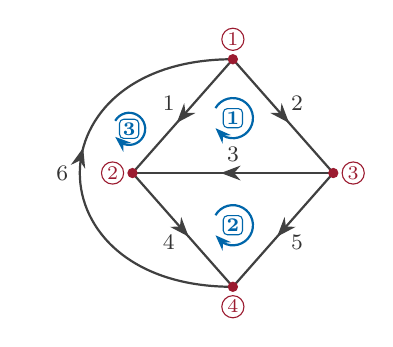
\begin{tikzpicture}[scale=0.85]
        \bridgecoords \bridgegraph \bridgemeshes
      \end{tikzpicture}\\[4pt]
      {\small $n = 4$, \ $b = 6$}
    \end{column}
    \begin{column}{0.62\textwidth}
      \centering
      Incidence matrix (rows: nodes \nd1, \nd2, \nd3)\\[4pt]
      $A =$\hspace{0.6em}\incmat{Ar}{6}{1,2,3}{%
         1 \&  1 \&  0 \&  0 \&  0 \& -1\\
        -1 \&  0 \& -1 \&  1 \&  0 \&  0\\
         0 \& -1 \&  1 \&  0 \&  1 \&  0\\}{}\\[6pt]
      Mesh matrix (rows: meshes \mlab1, \mlab2, \mlab3)\\[4pt]
      $M =$\hspace{0.6em}\incmatm{Mr}{6}{1,2,3}{%
        -1 \& 1 \& 1 \& 0 \& 0 \& 0\\
         0 \& 0 \& -1 \& -1 \& 1 \& 0\\
         1 \& 0 \& 0 \& 1 \& 0 \& 1\\}
    \end{column}
  \end{columns}
  \vfill
  \begin{center}
    $n - 1 = 3$ independent KCL equations, \ $b - n + 1 = 3$ independent KVL equations\\[4pt]
    Every row of $A$ is orthogonal to every row of $M$: \ $AM^T = \mathbf{0}$
  \end{center}
\end{frame}

%--------------------------------------------------------------
\begin{frame}{Review: node voltages and mesh currents}
  \vfill
  \begin{center}
  \renewcommand{\arraystretch}{1.35}
  \begin{tabular}{@{}l l l@{}}
  \toprule
   & \textbf{node voltages} & \textbf{mesh currents}\\
  \midrule
  works for                & any connected graph       & \alert{planar, nonseparable}\\
  number of unknowns       & $n - 1$                   & $b - n + 1$\\
  holds automatically      & KVL: $\Vcol{\mathbf{v}} = A^T\Vcol{\mathbf{e}}$
                           & KCL: $\Icol{\mathbf{i}} = M^T\Icol{\mathbf{i}_M}$\\
  left to write            & KCL: $A\Icol{\mathbf{i}} = \mathbf{0}$
                           & KVL: $M\Vcol{\mathbf{v}} = \mathbf{0}$\\
  \bottomrule
  \end{tabular}
  \end{center}
  \vfill
  \begin{center}
    Tellegen: $\Icol{\mathbf{i}}^T\Vcol{\mathbf{v}} = 0$
  \end{center}
  \vfill
\end{frame}

%--------------------------------------------------------------
\begin{frame}{Why this lecture?}
  \vfill
  \begin{itemize}\itemsep10pt
    \item \textbf{So far:} node voltages ($A$) work for any connected graph, with one fixed
      reference node. Mesh currents ($M$) need a \alert{planar, nonseparable} graph.
    \item<2-> \textbf{Problem:} \alert{nonplanar} graphs have no meshes, and in
      \alert{separable} graphs a mesh may not be bounded by a single loop.
    \item<3-> \textbf{Goal of this lecture:} methods that also work for nonplanar and
      separable circuits --- for \alert{every} connected graph.
    \item<4-> \textbf{Idea:} pick a \alert{tree}. It gives both sides:
      \begin{itemize}
        \item \alert{fundamental cutsets} generalise the node equations: same $n - 1$
          count, but the tree can be chosen;
        \item \alert{fundamental loops} generalise the mesh equations: $b - n + 1$ of them,
          for every connected graph.
      \end{itemize}
  \end{itemize}
  \vfill
\end{frame}

%--------------------------------------------------------------
\begin{frame}[t]{Nonplanar circuits}
  \centering
  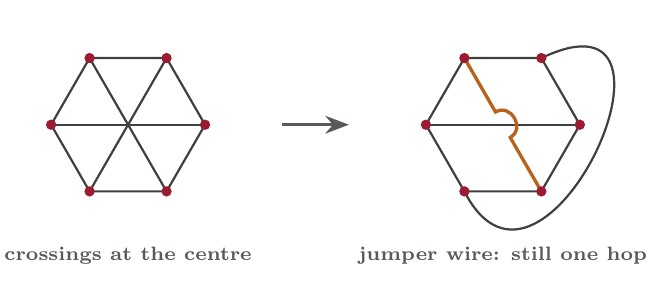
\begin{tikzpicture}[scale=0.85]
    \useasboundingbox (-1.5,-2.15) rectangle (7.6,1.45);
    \begin{scope}
      \foreach \a in {0,60,...,300} \coordinate (h\a) at (\a:1.15);
      \draw[black!75, thick] (h0) -- (h60) -- (h120) -- (h180) -- (h240) -- (h300) -- cycle;
      \draw[black!75, thick] (h0) -- (h180); \draw[black!75, thick] (h60) -- (h240);
      \draw[black!75, thick] (h120) -- (h300);
      \foreach \a in {0,60,...,300} \fill[metured] (h\a) circle (2.2pt);
      \node[ttl] at (0,-1.95) {crossings at the centre};
    \end{scope}
    \begin{scope}[visible on=<2->]
      \draw[bigarr] (2.3,0) -- (3.3,0);
      \begin{scope}[xshift=5.6cm]
        \hexhop
        \node[ttl] at (0,-1.95) {jumper wire: still one hop};
      \end{scope}
    \end{scope}
  \end{tikzpicture}\\[6pt]
  \only<1>{Can this graph be redrawn without crossings?}%
  \only<2->{No: at least one hop remains $\Rightarrow$ \alert{no meshes}, no mesh matrix.}\\[8pt]
  \onslide<3->{%
  \begin{block}{Question}
    Without meshes, how do we find $n-1$ independent KCL and $b-n+1$ independent KVL equations?\\
    Today: a method that needs \alert{no planar drawing} and works for \alert{any connected graph}.
  \end{block}}
\end{frame}

%--------------------------------------------------------------
\roadmapframe{1}

%--------------------------------------------------------------
\begin{frame}[t]{Trees}
  \begin{block}{Tree}
    A subgraph $T$ of a connected graph $G$ is a \alert{tree} if it contains all the nodes of
    $G$, is connected, and contains no loops.
  \end{block}
  \vspace{4pt}
  \begin{center}
  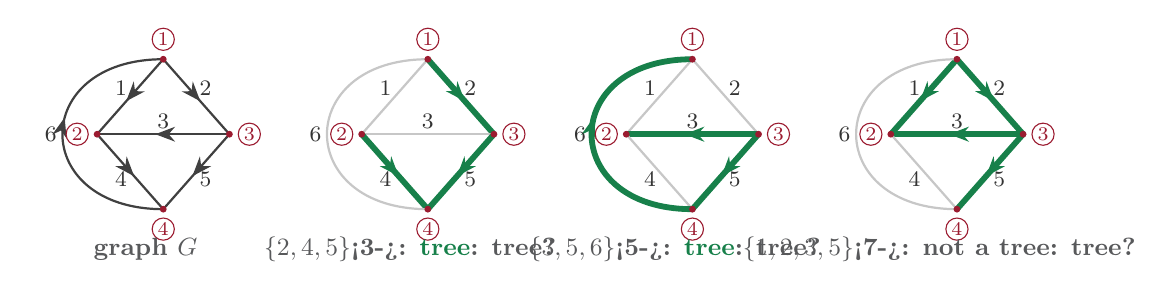
\begin{tikzpicture}[scale=0.56]
    \begin{scope}
      \bridgecoords \bridgegraph
      \node[ttl, font=\small\bfseries] at (-0.4,-2.6) {graph $G$};
    \end{scope}
    \begin{scope}[xshift=6.0cm, visible on=<2->]
      \bridgecoords \bridgesub{faintbr}{treebr}{faintbr}{treebr}{treebr}{faintbr}
      \node[ttl, font=\small\bfseries] at (-0.4,-2.6) {$\{2, 4, 5\}$\alt<3->{: \textcolor{ctree}{tree}}{: tree?}};
    \end{scope}
    \begin{scope}[xshift=12.0cm, visible on=<4->]
      \bridgecoords \bridgesub{faintbr}{faintbr}{treebr}{faintbr}{treebr}{treebr}
      \node[ttl, font=\small\bfseries] at (-0.4,-2.6) {$\{3, 5, 6\}$\alt<5->{: \textcolor{ctree}{tree}}{: tree?}};
    \end{scope}
    \begin{scope}[xshift=18.0cm, visible on=<6->]
      \bridgecoords \bridgesub{treebr}{treebr}{treebr}{faintbr}{treebr}{faintbr}
      \node[ttl, font=\small\bfseries] at (-0.4,-2.6) {$\{1, 2, 3, 5\}$\alt<7->{: \alert{not a tree}}{: tree?}};
    \end{scope}
  \end{tikzpicture}
  \end{center}
  \vfill
  \begin{center}
    \only<7->{Branches 1, 2, 3 form a loop. \ A graph has many trees.}
  \end{center}
\end{frame}

%--------------------------------------------------------------
\begin{frame}{How many branches does a tree have?}
  \vfill
  \begin{columns}[c,onlytextwidth]
    \begin{column}{0.55\textwidth}
      \begin{itemize}\itemsep6pt
        \item<2-> Start from one node; add tree branches one at a time.
        \item<3-> Each new branch must reach a \alert{new} node --- otherwise it closes a loop.
        \item<6-> Each branch adds one node. All $n$ nodes are reached after
          \alert{$n - 1$ branches}.
      \end{itemize}
      \vspace{8pt}
      \onslide<7->{The other \alert{$b - n + 1$} branches are left out.}
    \end{column}
    \begin{column}{0.4\textwidth}
      \centering
      \tikzset{reached/.style={fill=ctree!25}}
      \begin{tikzpicture}[scale=0.85]
        \bridgecoords
        \foreach \k/\p in {1/2-, 3/3-, 4/4-, 2/5-}
          \fill[reached, visible on=<\p>] (n\k) circle (0.24);
        \only<1-2>{\bridgesub{faintbr}{faintbr}{faintbr}{faintbr}{faintbr}{faintbr}}%
        \only<3>{\bridgesub{faintbr}{treebr}{faintbr}{faintbr}{faintbr}{faintbr}}%
        \only<4>{\bridgesub{faintbr}{treebr}{faintbr}{faintbr}{treebr}{faintbr}}%
        \only<5->{\bridgesub{faintbr}{treebr}{faintbr}{treebr}{treebr}{faintbr}}%
      \end{tikzpicture}\\[2pt]
      {\small
      \only<1>{$n = 4$ nodes, \ $b = 6$ branches}%
      \only<2>{start at node \nd1}%
      \only<3>{branch 2 reaches node \nd3}%
      \only<4>{branch 5 reaches node \nd4}%
      \only<5>{branch 4 reaches node \nd2}%
      \only<6>{4 nodes, 3 tree branches: \ $n - 1 = 3$}%
      \only<7->{left out: 1, 3, 6 \ ($b - n + 1 = 3$)}}
    \end{column}
  \end{columns}
  \vfill
\end{frame}

%--------------------------------------------------------------
\roadmapframe{2}

%--------------------------------------------------------------
\begin{frame}[t]{Cutsets}
  \begin{block}{Cutset}
    A set $C$ of branches of a connected graph is a \alert{cutset} if
    \begin{enumerate}
      \item removing \alert{all} of $C$ leaves the graph \alert{unconnected}, and
      \item after removing $C$, putting back \alert{a single} branch of $C$ makes it
            \alert{connected} again --- \alert{whichever} branch we put back.
    \end{enumerate}
  \end{block}
  \vfill
  \begin{center}
  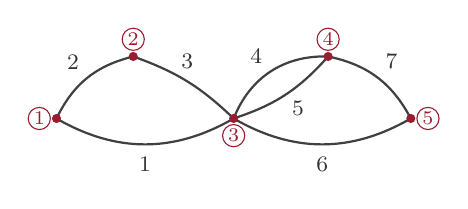
\begin{tikzpicture}[scale=0.75]
    \eightcoords
    \eightsub{plainbr}{plainbr}{plainbr}{plainbr}{plainbr}{plainbr}{plainbr}
  \end{tikzpicture}
  \end{center}
  \vfill
  \begin{center}
    \onslide<2->{In words: removing $C$ gives \alert{two pieces}, and \alert{every} branch of $C$ is needed.}\\[3pt]
    \onslide<3->{Picture: a \alert{closed surface} around one piece crosses
      \alert{exactly} the branches of the cutset.}
  \end{center}
  \vfill
\end{frame}

%--------------------------------------------------------------
\begin{frame}{Example: cutsets}
  \tikzset{backbr/.style={ctree, line width=2.2pt}}
  \newcommand{\yes}{\textcolor{ctree}{\checkmark}}
  \begin{columns}[c,onlytextwidth]
    \begin{column}{0.52\textwidth}
      \centering
      \begin{tikzpicture}[scale=0.86]
        \useasboundingbox (-3.75,-1.0) rectangle (3.75,1.75);
        \eightcoords
        \only<1>{\eightsub{plainbr}{plainbr}{plainbr}{cutbr}{cutbr}{plainbr}{cutbr}}
        \only<2>{\pieceP \eightsub{plainbr}{plainbr}{plainbr}{cutaway}{cutaway}{plainbr}{cutaway}}
        \only<3>{\eightsub{plainbr}{plainbr}{plainbr}{backbr}{cutaway}{plainbr}{cutaway}}
        \only<4>{\eightsub{plainbr}{plainbr}{plainbr}{cutbr}{cutbr}{plainbr}{cutbr} \pieceP[fill=none]}
        \only<5>{\eightsub{cutbr}{plainbr}{cutbr}{plainbr}{plainbr}{plainbr}{plainbr}}
        \only<6>{\pieceLT \eightsub{cutaway}{plainbr}{cutaway}{plainbr}{plainbr}{plainbr}{plainbr}}
        \only<7>{\eightsub{plainbr}{plainbr}{plainbr}{plainbr}{plainbr}{cutbr}{cutbr}}
        \only<8>{\pieceR \eightsub{plainbr}{plainbr}{plainbr}{plainbr}{plainbr}{cutaway}{cutaway}}
      \end{tikzpicture}
    \end{column}
    \begin{column}{0.46\textwidth}
      \only<1-4>{%
        $C_1 = \{\textcolor{cvolt}{4, 5, 7}\}$\\[8pt]
        \onslide<2->{(1) Remove all three: node \nd4 is cut off. \yes\\[6pt]}
        \onslide<3->{(2) Put back one, e.g.\ \textcolor{ctree}{4}: node \nd4 is reached again.
          Same for 5 or 7. \yes\\[8pt]
          $\Rightarrow$ $C_1$ is a \alert{cutset}.}}%
      \only<5-6>{%
        $C_2 = \{\textcolor{cvolt}{1, 3}\}$\\[8pt]
        \onslide<6->{(1) Remove both: nodes \nd1, \nd2 are cut off. \yes\\[6pt]
          (2) Put back 1 or 3: connected again. \yes\\[8pt]
          $\Rightarrow$ $C_2$ is a \alert{cutset}.}}%
      \only<7-8>{%
        $C_3 = \{\textcolor{cvolt}{6, 7}\}$\\[8pt]
        \onslide<8->{(1) Remove both: node \nd5 is cut off. \yes\\[6pt]
          (2) Put back 6 or 7: connected again. \yes\\[8pt]
          $\Rightarrow$ $C_3$ is a \alert{cutset}.}}
    \end{column}
  \end{columns}
  \vfill
  \begin{center}\small
    \only<1-3,5-7>{\phantom{X}}%
    \only<4>{All branches back: the closed surface around node \nd4 crosses
      \alert{exactly} 4, 5, 7.}%
    \only<8>{Cutsets can have \alert{different sizes}: $C_1$ has 3 branches, $C_2$ and $C_3$
      have 2.}
  \end{center}
\end{frame}

%--------------------------------------------------------------
\begin{frame}{Example: not every set is a cutset}
  \tikzset{backbr/.style={ctree, line width=2.2pt}}
  \newcommand{\yes}{\textcolor{ctree}{\checkmark}}
  \newcommand{\no}{\textcolor{metured}{$\boldsymbol{\times}$}}
  \begin{columns}[c,onlytextwidth]
    \begin{column}{0.52\textwidth}
      \centering
      \begin{tikzpicture}[scale=0.86]
        \useasboundingbox (-3.75,-1.0) rectangle (3.75,1.75);
        \eightcoords
        \only<1>{\eightsub{cutbr}{plainbr}{cutbr}{cutbr}{cutbr}{cutbr}{plainbr}}
        \only<2>{\pieceLT \pieceM \piecePR
          \eightsub{cutaway}{plainbr}{cutaway}{cutaway}{cutaway}{cutaway}{plainbr}}
        \only<3>{\pieceLTM \piecePR
          \eightsub{backbr}{plainbr}{cutaway}{cutaway}{cutaway}{cutaway}{plainbr}}
        \only<4>{\pieceLTM \piecePR
          \eightsub{plainbr}{plainbr}{plainbr}{cutaway}{cutaway}{cutaway}{plainbr}}
        \only<5>{\eightsub{plainbr}{plainbr}{plainbr}{cutbr}{plainbr}{cutbr}{plainbr}}
        \only<6>{\eightsub{plainbr}{plainbr}{plainbr}{cutaway}{plainbr}{cutaway}{plainbr}}
        \only<7>{\piecePR[fill=none]
          \eightsub{plainbr}{plainbr}{plainbr}{cutbr}{cutbr}{cutbr}{plainbr}}
        \only<8>{\eightsub{cutbr}{plainbr}{plainbr}{cutbr}{cutbr}{plainbr}{cutbr}}
        \only<9>{\pieceP
          \eightsub{cutaway}{plainbr}{plainbr}{cutaway}{cutaway}{plainbr}{cutaway}}
        \only<10>{\eightsub{cutaway}{plainbr}{plainbr}{backbr}{cutaway}{plainbr}{cutaway}}
        \only<11>{\pieceP
          \eightsub{backbr}{plainbr}{plainbr}{cutaway}{cutaway}{plainbr}{cutaway}}
      \end{tikzpicture}
    \end{column}
    \begin{column}{0.46\textwidth}
      \only<1-4>{%
      $C = \{\textcolor{cvolt}{1, 3, 4, 5, 6}\}$: a cutset?\\[8pt]
      \onslide<2->{(1) Remove all five: \alert{three} pieces. \yes\\[6pt]}
      \onslide<3->{(2) Put back \textcolor{ctree}{1}: still unconnected. \no\\[8pt]
        $\Rightarrow$ \alert{not} a cutset: some branches are not needed.\\[8pt]}
      \onslide<4->{Branches 1, 3 are extra: $\{4, 5, 6\}$ alone is a cutset.}}%
      \only<5-7>{%
      $C = \{\textcolor{cvolt}{4, 6}\}$: a cutset?\\[8pt]
      \onslide<6->{(1) Remove both: still \alert{one} piece --- branch 5 still joins \nd3
        and \nd4. \no\\[6pt]
        $\Rightarrow$ \alert{not} a cutset: a branch is missing.\\[8pt]}
      \onslide<7->{Branches 4 and 5 both join \nd3 and \nd4 (\alert{parallel}): a surface
        that crosses one crosses the other. Here the surface gives $\{4, 5, 6\}$.}}%
      \only<8-11>{%
      $C = \{\textcolor{cvolt}{1, 4, 5, 7}\}$: a cutset?\\[8pt]
      \onslide<9->{(1) Remove all four: node \nd4 cut off, \alert{two} pieces. \yes\\[6pt]}
      \onslide<10->{(2) Put back \textcolor{ctree}{4}, 5 or 7: connected. \yes\\[6pt]}
      \onslide<11->{\phantom{(2)} Put back \textcolor{ctree}{1}: still unconnected. \no\\[8pt]
        $\Rightarrow$ \alert{not} a cutset: (2) must hold \alert{whichever} branch we put back.
        Branch 1 is not needed: $\{4, 5, 7\}$ is a cutset.}}
    \end{column}
  \end{columns}
\end{frame}

%--------------------------------------------------------------
\begin{frame}{KCL on a cutset}
  \newcommand{\yes}{\textcolor{ctree}{\checkmark}}
  \begin{columns}[c,onlytextwidth]
    \begin{column}{0.52\textwidth}
      \centering
      \begin{tikzpicture}[scale=0.86]
        \useasboundingbox (-3.75,-1.0) rectangle (3.75,1.75);
        \eightcoords
        \only<2>{\piecePR}
        \only<1>{\eightI{plainbr}{plainbr}{plainbr}{plainbr}{plainbr}{plainbr}{plainbr}}%
        \only<2>{\eightI{plainbr}{plainbr}{plainbr}{cutbr}{cutbr}{cutbr}{plainbr}}%
      \end{tikzpicture}\\[6pt]
      \eightItable
    \end{column}
    \begin{column}{0.46\textwidth}
      \only<1>{Branch currents in the arrow directions.\\[6pt]
        They satisfy KCL at every node, e.g.\ node \nd3:
        \[\Ik1 + \Ik4 + \Ik5 - \Ik3 - \Ik6 = 2 + 1 + 2 - 2 - 3 = 0.\]}%
      \only<2>{Cutset $\{\textcolor{cvolt}{4, 5, 6}\}$: surface around \nd4, \nd5\\[4pt]
        leaving: \Ik6; \ entering: \Ik4, \Ik5
        \[\Ik6 - \Ik4 - \Ik5 = 3 - 1 - 2 = 0 \ \yes\]
        {\small KCL at \nd4: \ $\Ik7 - \Ik4 - \Ik5 = 0$\\
        KCL at \nd5: \ $\Ik6 - \Ik7 = 0$\\[3pt]
        Add them: \Ik7 is inside the surface and cancels.}}
    \end{column}
  \end{columns}
  \vfill
  \begin{center}
    \onslide<2->{\alert{KCL on a cutset:} the cutset currents add up to zero\\
      {\small ($+$ leaving the surface, $-$ entering).}}
  \end{center}
\end{frame}

%--------------------------------------------------------------
\roadmapframe{3}

%--------------------------------------------------------------
\begin{frame}[t]{Fundamental cutsets}
  \tikzset{partfill/.style={fill=ctree!13}}
  \begin{columns}[T,onlytextwidth]
    \begin{column}{0.44\textwidth}
      \centering
      \begin{tikzpicture}[scale=1.05]
        \useasboundingbox (-2.6,-0.75) rectangle (2.5,2.75);
        \tgcoords
        \only<1>{\tgtree}%
        \only<2>{\tgraph{treebr}{cotreebr}{hlbr}{cotreebr}{cotreebr}{treebr}}%
        \only<3>{\fill[partfill] (0,1.8) ellipse (1.55 and 0.5);
          \fill[partfill] (-1,0) ellipse (1.4 and 0.42);
          \tgraph{treebr}{faintbr}{cutaway}{faintbr}{faintbr}{treebr}}%
        \only<4>{\fill[partfill] (0,1.8) ellipse (1.55 and 0.5);
          \fill[partfill] (-1,0) ellipse (1.4 and 0.42);
          \draw[surf] (0,1.8) ellipse (1.8 and 0.8);
          \tgraph{treebr}{hlbr}{hlbr}{hlbr}{hlbr}{treebr}}%
      \end{tikzpicture}\\[2pt]
      {\small tree \textcolor{ctree}{$\{1, 3, 6\}$}, \ co-tree $\{2, 4, 5\}$}
    \end{column}
    \begin{column}{0.54\textwidth}
      \begin{enumerate}\itemsep3pt
        \item<1-> Fix a \alert{tree} (green). The other branches form the \alert{co-tree}.
        \item<2-> Pick one tree branch, e.g.\ \textcolor{cvolt}{3}.
        \item<3-> Remove it: the tree falls into \alert{two parts},
          $\{\nd1, \nd2\}$ and $\{\nd3, \nd4\}$.
        \item<4-> The branches joining the two parts form a cutset:
          $\{\textcolor{cvolt}{3, 2, 4, 5}\}$. It is the \alert{fundamental cutset} of 3.
      \end{enumerate}
    \end{column}
  \end{columns}
\end{frame}

%--------------------------------------------------------------
\begin{frame}[t]{Fundamental cutset: one tree branch, one direction}
  \tikzset{partfill/.style={fill=ctree!13}}
  \begin{columns}[T,onlytextwidth]
    \begin{column}{0.46\textwidth}
      \centering
      \begin{tikzpicture}[scale=0.85]
        \useasboundingbox (-2.75,-0.75) rectangle (2.75,3.15);
        \tgcoords
        \fill[partfill] (0,1.8) ellipse (1.55 and 0.5);
        \fill[partfill] (-1,0) ellipse (1.4 and 0.42);
        \draw[surf] (0,1.8) ellipse (1.8 and 0.8);
        \tgraph{treebr}{hlbr}{treebr}{hlbr}{hlbr}{treebr}
        \node[font=\scriptsize, text=ctree, anchor=east] at (-1.75,2.6) {part $\{\nd1, \nd2\}$};
        \node[font=\scriptsize, text=ctree] at (0,-0.75) {part $\{\nd3, \nd4\}$};
        \begin{scope}[visible on=<2->]
          \foreach \t in {30,90,150,210,330,-90} {
            \pgfmathsetmacro{\nx}{cos(\t)/1.8} \pgfmathsetmacro{\ny}{sin(\t)/0.8}
            \pgfmathsetmacro{\nn}{sqrt(\nx*\nx+\ny*\ny)}
            \draw[-{Stealth[length=2.4mm]}, cvolt, line width=1.3pt]
              ({1.8*cos(\t)},{1.8+0.8*sin(\t)}) -- ++({0.4*\nx/\nn},{0.4*\ny/\nn});}
          \node[font=\scriptsize, text=cvolt] at (0.9,3.0) {cutset direction: out};
        \end{scope}
      \end{tikzpicture}\\[2pt]
      \onslide<4->{%
      \begin{block}{Fundamental cutset}
        \small
        \begin{itemize}
          \item the tree branch $+$ the co-tree branches joining the two parts
          \item only \alert{one} tree branch in it
          \item direction: that of the tree branch
        \end{itemize}
      \end{block}}
    \end{column}
    \begin{column}{0.52\textwidth}
      Cutset of 3: $\{3, 2, 4, 5\}$\\[4pt]
      \textbf{One tree branch.} Only \textcolor{ctree}{3} is a tree branch; 2, 4, 5 are
      co-tree branches. The other tree branches (1, 6) lie \alert{inside one part}.\\[5pt]
      \onslide<2->{\textbf{Direction.} Branch 3 \alert{leaves} the surface, from part
        $\{\nd1, \nd2\}$ to part $\{\nd3, \nd4\}$: the cutset points \alert{out}.\\[5pt]}
      \onslide<3->{\textbf{KCL.} Branch $k$ carries current \Icol{$i_k$} along its arrow.
        KCL on the surface: $+$ leaving, $-$ entering. Branches 2, 4, 5 leave too:
        \[\Icol{i_3} + \Icol{i_2} + \Icol{i_4} + \Icol{i_5} = 0.\]}
    \end{column}
  \end{columns}
\end{frame}

%--------------------------------------------------------------
\begin{frame}[t]{Example: fundamental cutsets of $G$}
  \vspace{4pt}
  \begin{columns}[T,onlytextwidth]
    \begin{column}{0.44\textwidth}
      \centering
      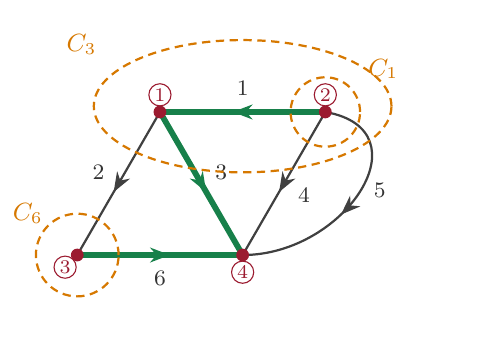
\begin{tikzpicture}[scale=1.05]
        \useasboundingbox (-2.6,-0.75) rectangle (2.5,2.75);
        \tgcoords \tgtree
        \begin{scope}[visible on=<2->]
          \draw[surf] (g2) circle (0.42);  \node[font=\small, text=cvolt] at (1.7,2.25) {$C_1$};
        \end{scope}
        \begin{scope}[visible on=<3->]
          \draw[surf] (0,1.8) ellipse (1.8 and 0.8); \node[font=\small, text=cvolt] at (-1.95,2.55) {$C_3$};
        \end{scope}
        \begin{scope}[visible on=<4->]
          \draw[surf] (g3) circle (0.5);   \node[font=\small, text=cvolt] at (-2.6,0.5) {$C_6$};
        \end{scope}
      \end{tikzpicture}
    \end{column}
    \begin{column}{0.54\textwidth}
      \small
      For each tree branch: its fundamental cutset, and \alert{KCL on that cutset}
      (branch currents \Icol{$i_k$} along the arrows; $+$ if a branch crosses the surface the
      same way as the tree branch, $-$ if not).
      \\[6pt]
      \renewcommand{\arraystretch}{1.3}
      \begin{tabular}{@{}c l l@{}}
        tree br. & cutset & KCL on it\\ \hline
        \uncover<2->{1} & \uncover<2->{$\{1, 4, 5\}$}    & \uncover<2->{$\Icol{i_1} + \Icol{i_4} + \Icol{i_5} = 0$}\\
        \uncover<3->{3} & \uncover<3->{$\{3, 2, 4, 5\}$} & \uncover<3->{$\Icol{i_3} + \Icol{i_2} + \Icol{i_4} + \Icol{i_5} = 0$}\\
        \uncover<4->{6} & \uncover<4->{$\{6, 2\}$}       & \uncover<4->{$\Icol{i_6} - \Icol{i_2} = 0$}
      \end{tabular}\\[8pt]
      \onslide<5->{\alert{$n - 1 = 3$ KCL equations, independent:} each has its own tree
        branch current.}
    \end{column}
  \end{columns}
\end{frame}

%--------------------------------------------------------------
\begin{frame}[t]{Matrix form: fundamental cutset matrix $Q$}
  \begin{columns}[T,onlytextwidth]
    \begin{column}{0.36\textwidth}
      \centering
      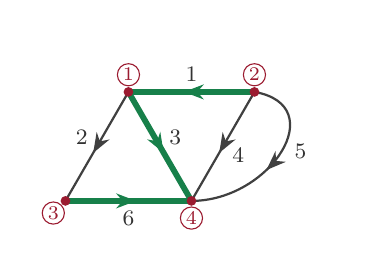
\begin{tikzpicture}[scale=0.8]
        \useasboundingbox (-2.6,-0.75) rectangle (2.5,2.75);
        \tgcoords \tgtree
      \end{tikzpicture}\\[2pt]
      {\small tree \textcolor{ctree}{$\{1, 3, 6\}$}}
    \end{column}
    \begin{column}{0.62\textwidth}
      Collect the fundamental cutset KCL equations in a matrix:\\[4pt]
      {\small one \alert{row} per tree branch, one \alert{column} per branch;\\
        $+1$ / $-1$: branch in the cutset, same / opposite direction; \ $0$: not in it.}
      \[
        Q = \brmat{Qm}{1, 3, 6}{\Qrows}{%
          \foreach \j in {1,3,6} {\begin{scope}[visible on=<3->]\colbox{Qm}{\j}{ctree}\end{scope}}}
      \]
      \onslide<2->{KCL: \ \alert{$Q\Icol{\mathbf{i}} = \mathbf{0}$} \quad (like
        $A\Icol{\mathbf{i}} = \mathbf{0}$)\\[6pt]}
      \onslide<3->{\small Tree columns 1, 3, 6 form an \alert{identity}: each row has its own
        tree branch, so the rows are independent.}
    \end{column}
  \end{columns}
\end{frame}

%--------------------------------------------------------------
\begin{frame}[t]{Branch currents from co-tree currents}
  \begin{columns}[T,onlytextwidth]
    \begin{column}{0.4\textwidth}
      \centering
      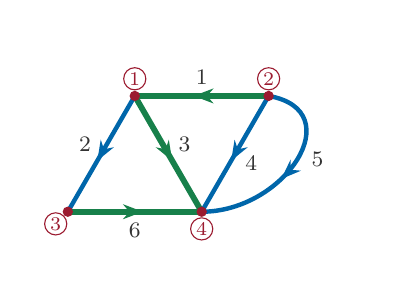
\begin{tikzpicture}[scale=0.85]
        \useasboundingbox (-2.6,-0.75) rectangle (2.5,2.75);
        \tgcoords
        \tgraph{treebr}{gbr, ccur, line width=1.6pt}{treebr}{gbr, ccur, line width=1.6pt}{gbr, ccur, line width=1.6pt}{treebr}
      \end{tikzpicture}\\[2pt]
      {\small tree \textcolor{ctree}{$\{1, 3, 6\}$}, \ co-tree \Icol{$\{2, 4, 5\}$}}
    \end{column}
    \begin{column}{0.58\textwidth}
      \textbf{Goal.} Relate \alert{every} branch current to the \Icol{co-tree} currents
      $\Icol{i_2}, \Icol{i_4}, \Icol{i_5}$.\\[8pt]
      \onslide<2->{\textbf{Co-tree branches:} nothing to do --- $\Icol{i_2}, \Icol{i_4},
        \Icol{i_5}$ themselves.\\[6pt]}
      \onslide<3->{\textbf{Tree branches:} each fundamental cutset has \alert{one} tree
        branch. Solve its KCL for that current:
        \[\Icol{i_1} = -\Icol{i_4} - \Icol{i_5}, \quad
          \Icol{i_3} = -\Icol{i_2} - \Icol{i_4} - \Icol{i_5}, \quad
          \Icol{i_6} = \Icol{i_2}\]}
      \onslide<4->{So all $b$ branch currents are combinations of the $b - n + 1$ co-tree
        currents, and KCL holds automatically --- like mesh currents.}
    \end{column}
  \end{columns}
\end{frame}

%--------------------------------------------------------------
\begin{frame}{In matrix form: $\Icol{\mathbf{i}} = B^T\Icol{\mathbf{i}_C}$}
  \begin{center}
    Every branch current from the co-tree currents
    $\Icol{\mathbf{i}_C} = [\Icol{i_2}\ \Icol{i_4}\ \Icol{i_5}]^T$:
  \end{center}
  \begin{center}
    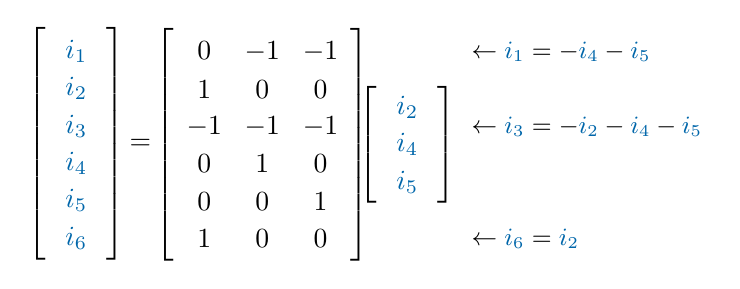
\begin{tikzpicture}[mm/.style={matrix of math nodes, ampersand replacement=\&,
        left delimiter={[}, right delimiter={]}, inner sep=1pt, column sep=0.4em,
        nodes={minimum height=1.35em, text width=1.5em, align=center, inner sep=1pt}}]
      \matrix (L) [mm] {\Icol{i_1} \\ \Icol{i_2} \\ \Icol{i_3} \\ \Icol{i_4} \\ \Icol{i_5} \\ \Icol{i_6} \\};
      \node (eq) [right=6pt of L] {$=$};
      \matrix (M) [mm, right=6pt of eq] {0 \& -1 \& -1 \\ 1 \& 0 \& 0 \\ -1 \& -1 \& -1 \\ 0 \& 1 \& 0 \\ 0 \& 0 \& 1 \\ 1 \& 0 \& 0 \\};
      \matrix (R) [mm, right=12pt of M] {\Icol{i_2} \\ \Icol{i_4} \\ \Icol{i_5} \\};
      \node[anchor=west, font=\small] at ([xshift=10pt]R.east |- M-1-3) {$\leftarrow \Icol{i_1} = -\Icol{i_4} - \Icol{i_5}$};
      \node[anchor=west, font=\small] at ([xshift=10pt]R.east |- M-3-3) {$\leftarrow \Icol{i_3} = -\Icol{i_2} - \Icol{i_4} - \Icol{i_5}$};
      \node[anchor=west, font=\small] at ([xshift=10pt]R.east |- M-6-3) {$\leftarrow \Icol{i_6} = \Icol{i_2}$};
    \end{tikzpicture}
  \end{center}
  \begin{center}
    \onslide<2->{We call this $6 \times 3$ matrix $B^T$: \quad \alert{$\Icol{\mathbf{i}} = B^T\Icol{\mathbf{i}_C}$},
      \ like $\Icol{\mathbf{i}} = M^T\Icol{\mathbf{i}_M}$. KCL holds for any $\Icol{\mathbf{i}_C}$.\\[6pt]}
    \onslide<3->{Its transpose $B$ (rows: co-tree branches 2, 4, 5) will appear again with the
      fundamental loops.}
  \end{center}
\end{frame}

%--------------------------------------------------------------
\roadmapframe{4}

%--------------------------------------------------------------
\begin{frame}[t]{Fundamental loops}
  \begin{columns}[T,onlytextwidth]
    \begin{column}{0.44\textwidth}
      \centering
      \begin{tikzpicture}[scale=0.85]
        \useasboundingbox (-2.6,-0.75) rectangle (2.5,2.75);
        \tgcoords
        \only<1>{\tgtree}%
        \only<2>{\tgraph{treebr}{faintbr}{treebr}{hlbr}{faintbr}{treebr}}%
        \only<3->{\tgraph{hlbr}{faintbr}{hlbr}{hlbr}{faintbr}{faintbr}}%
        \only<4->{\loopcw{0}{1.15}}%
      \end{tikzpicture}\\[4pt]
      \onslide<6->{%
      \begin{block}{Fundamental loop}
        \small
        \begin{itemize}
          \item the co-tree branch $+$ the tree path between its ends
          \item only \alert{one} co-tree branch in it
          \item direction: that of the co-tree branch
        \end{itemize}
      \end{block}}
    \end{column}
    \begin{column}{0.54\textwidth}
      \begin{enumerate}\itemsep3pt
        \item<1-> Fix a \alert{tree} (green): $\{1, 3, 6\}$. Co-tree: $\{2, 4, 5\}$.
        \item<2-> Pick one \alert{co-tree} branch, e.g.\ \textcolor{cvolt}{4}.
        \item<3-> Add it to the tree: it closes \alert{exactly one loop}, branch 4 plus the
          tree path between its ends (3 and 1).
        \item<4-> This loop $\{\textcolor{cvolt}{4, 3, 1}\}$ is the \alert{fundamental loop}
          of 4. Its direction is that of branch 4.
        \item<5-> KVL around it: $+\Vcol{v_k}$ along an arrow, $-\Vcol{v_k}$ against:
          \[\Vcol{v_4} - \Vcol{v_3} - \Vcol{v_1} = 0.\]
      \end{enumerate}
    \end{column}
  \end{columns}
\end{frame}

%--------------------------------------------------------------
\begin{frame}[t]{Example: fundamental loops of $G$}
  \vspace{4pt}
  \begin{columns}[T,onlytextwidth]
    \begin{column}{0.44\textwidth}
      \centering
      \begin{tikzpicture}[scale=1.05]
        \useasboundingbox (-2.6,-0.75) rectangle (2.5,2.75);
        \tgcoords
        \only<1>{\tgtree}%
        \only<2>{\tgraph{faintbr}{hlbr}{hlbr}{faintbr}{faintbr}{hlbr}\loopccw{-1}{0.6}}%
        \only<3>{\tgraph{hlbr}{faintbr}{hlbr}{hlbr}{faintbr}{faintbr}\loopcw{0}{1.15}}%
        \only<4->{\tgraph{hlbr}{faintbr}{hlbr}{faintbr}{hlbr}{faintbr}\loopcw[0.25]{0}{1.2}}%
      \end{tikzpicture}\\[2pt]
      {\small tree $\{1, 3, 6\}$, co-tree $\{2, 4, 5\}$}
    \end{column}
    \begin{column}{0.54\textwidth}
      \small
      For each co-tree branch: its fundamental loop, and \alert{KVL around it} (walk in the
      direction of the co-tree branch; $+\Vcol{v_k}$ along an arrow, $-\Vcol{v_k}$ against).
      \\[6pt]
      \renewcommand{\arraystretch}{1.35}
      \begin{tabular}{@{}c l l@{}}
        co-tree br. & loop & KVL around it\\ \hline
        \uncover<2->{2} & \uncover<2->{$\{2, 6, 3\}$}    & \uncover<2->{$\Vcol{v_2} + \Vcol{v_6} - \Vcol{v_3} = 0$}\\
        \uncover<3->{4} & \uncover<3->{$\{4, 3, 1\}$}    & \uncover<3->{$\Vcol{v_4} - \Vcol{v_3} - \Vcol{v_1} = 0$}\\
        \uncover<4->{5} & \uncover<4->{$\{5, 3, 1\}$} & \uncover<4->{$\Vcol{v_5} - \Vcol{v_3} - \Vcol{v_1} = 0$}
      \end{tabular}\\[10pt]
      \onslide<5->{\alert{$b - n + 1 = 3$ KVL equations, independent:} each has its own
        co-tree branch voltage.}
    \end{column}
  \end{columns}
\end{frame}

%--------------------------------------------------------------
\begin{frame}[t]{Matrix form: fundamental loop matrix $B$}
  \begin{columns}[T,onlytextwidth]
    \begin{column}{0.36\textwidth}
      \centering
      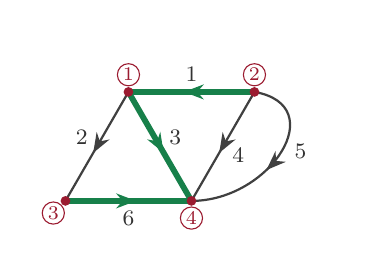
\begin{tikzpicture}[scale=0.8]
        \useasboundingbox (-2.6,-0.75) rectangle (2.5,2.75);
        \tgcoords \tgtree
      \end{tikzpicture}\\[2pt]
      {\small co-tree $\{2, 4, 5\}$}
    \end{column}
    \begin{column}{0.62\textwidth}
      Collect the fundamental loop KVL equations in a matrix:\\[4pt]
      {\small one \alert{row} per co-tree branch, one \alert{column} per branch;\\
        $+1$ / $-1$: branch in the loop, along / against its direction; \ $0$: not in it.}
      \[
        B = \brmat{Bm}{2, 4, 5}{\Brows}{%
          \foreach \j in {2,4,5} {\begin{scope}[visible on=<3->]\colbox{Bm}{\j}{cvolt}\end{scope}}}
      \]
      \onslide<2->{KVL: \ \alert{$B\Vcol{\mathbf{v}} = \mathbf{0}$} \quad (like
        $M\Vcol{\mathbf{v}} = \mathbf{0}$)\\[6pt]}
      \onslide<3->{\small Co-tree columns 2, 4, 5 form an \alert{identity}: each row has its
        own co-tree branch, so the rows are independent.\\}
      \onslide<4->{\small Compare with $\Icol{\mathbf{i}} = B^T\Icol{\mathbf{i}_C}$: the
        \alert{same} matrix $B$.}
    \end{column}
  \end{columns}
\end{frame}

%--------------------------------------------------------------
\begin{frame}[t]{Branch voltages from tree voltages}
  \begin{columns}[T,onlytextwidth]
    \begin{column}{0.4\textwidth}
      \centering
      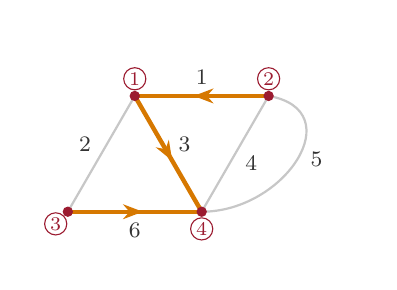
\begin{tikzpicture}[scale=0.85]
        \useasboundingbox (-2.6,-0.75) rectangle (2.5,2.75);
        \tgcoords
        \tgraph{gbr, cvolt, line width=1.6pt}{faintbr}{gbr, cvolt, line width=1.6pt}{faintbr}{faintbr}{gbr, cvolt, line width=1.6pt}
      \end{tikzpicture}\\[2pt]
      {\small tree \Vcol{$\{1, 3, 6\}$}, \ co-tree $\{2, 4, 5\}$}
    \end{column}
    \begin{column}{0.58\textwidth}
      \textbf{Goal.} Relate \alert{every} branch voltage to the \Vcol{tree} voltages
      $\Vcol{v_1}, \Vcol{v_3}, \Vcol{v_6}$.\\[8pt]
      \onslide<2->{\textbf{Tree branches:} nothing to do --- $\Vcol{v_1}, \Vcol{v_3},
        \Vcol{v_6}$ themselves.\\[6pt]}
      \onslide<3->{\textbf{Co-tree branches:} each fundamental loop has \alert{one} co-tree
        branch. Solve its KVL for that voltage:
        \[\Vcol{v_2} = \Vcol{v_3} - \Vcol{v_6}, \quad
          \Vcol{v_4} = \Vcol{v_1} + \Vcol{v_3}, \quad
          \Vcol{v_5} = \Vcol{v_1} + \Vcol{v_3}\]}
      \onslide<4->{So all $b$ branch voltages are combinations of the $n - 1$ tree voltages,
        and KVL holds automatically --- like node voltages.}
    \end{column}
  \end{columns}
\end{frame}

%--------------------------------------------------------------
\begin{frame}{In matrix form: $\Vcol{\mathbf{v}} = Q^T\Vcol{\mathbf{v}_T}$}
  \begin{center}
    Every branch voltage from the tree voltages
    $\Vcol{\mathbf{v}_T} = [\Vcol{v_1}\ \Vcol{v_3}\ \Vcol{v_6}]^T$:
  \end{center}
  \begin{center}
    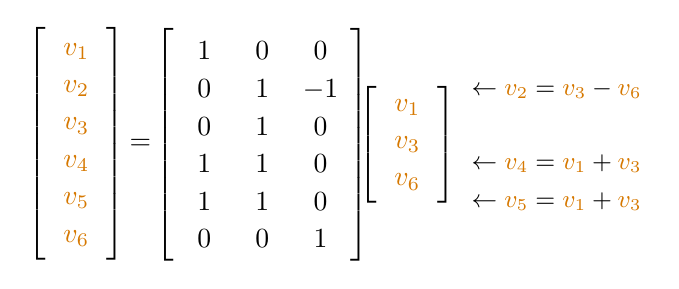
\begin{tikzpicture}[mm/.style={matrix of math nodes, ampersand replacement=\&,
        left delimiter={[}, right delimiter={]}, inner sep=1pt, column sep=0.4em,
        nodes={minimum height=1.35em, text width=1.5em, align=center, inner sep=1pt}}]
      \matrix (L) [mm] {\Vcol{v_1} \\ \Vcol{v_2} \\ \Vcol{v_3} \\ \Vcol{v_4} \\ \Vcol{v_5} \\ \Vcol{v_6} \\};
      \node (eq) [right=6pt of L] {$=$};
      \matrix (M) [mm, right=6pt of eq] {1 \& 0 \& 0 \\ 0 \& 1 \& -1 \\ 0 \& 1 \& 0 \\ 1 \& 1 \& 0 \\ 1 \& 1 \& 0 \\ 0 \& 0 \& 1 \\};
      \matrix (R) [mm, right=12pt of M] {\Vcol{v_1} \\ \Vcol{v_3} \\ \Vcol{v_6} \\};
      \node[anchor=west, font=\small] at ([xshift=10pt]R.east |- M-2-3) {$\leftarrow \Vcol{v_2} = \Vcol{v_3} - \Vcol{v_6}$};
      \node[anchor=west, font=\small] at ([xshift=10pt]R.east |- M-4-3) {$\leftarrow \Vcol{v_4} = \Vcol{v_1} + \Vcol{v_3}$};
      \node[anchor=west, font=\small] at ([xshift=10pt]R.east |- M-5-3) {$\leftarrow \Vcol{v_5} = \Vcol{v_1} + \Vcol{v_3}$};
    \end{tikzpicture}
  \end{center}
  \begin{center}
    \onslide<2->{This matrix is $Q^T$, the transpose of the fundamental cutset matrix:
      \alert{$\Vcol{\mathbf{v}} = Q^T\Vcol{\mathbf{v}_T}$}, like
      $\Vcol{\mathbf{v}} = A^T\Vcol{\mathbf{e}}$. KVL holds for any $\Vcol{\mathbf{v}_T}$.\\[6pt]}
    \onslide<3->{And the two matrices fit together: \alert{$QB^T = \mathbf{0}$}, like
      $AM^T = \mathbf{0}$.}
  \end{center}
\end{frame}
%--------------------------------------------------------------
\roadmapframe{5}

%--------------------------------------------------------------
\begin{frame}{Any connected graph}
  \vfill
  \begin{center}
    \renewcommand{\arraystretch}{1.3}
    \begin{tabular}{@{}l c l@{}}
      \toprule
       & how many & gives\\
      \midrule
      tree branches   & $n - 1$     & fundamental cutsets: the KCL equations\\
      co-tree branches & $b - n + 1$ & fundamental loops: the KVL equations\\
      \bottomrule
    \end{tabular}
  \end{center}
  \vfill
  \begin{center}
    \onslide<2->{No drawing needed: works for \alert{nonplanar} graphs.\\[6pt]}
    \onslide<3->{It also works for \alert{separable} graphs. Example next.}
  \end{center}
  \vfill
\end{frame}

%--------------------------------------------------------------
\begin{frame}[t]{Example: the separable graph}
  \begin{columns}[T,onlytextwidth]
    \begin{column}{0.4\textwidth}
      \centering
      \begin{tikzpicture}[scale=1.3]
        \useasboundingbox (-0.6,-0.6) rectangle (3.0,3.0);
        \sepcoords
        \only<1>{\sepgraph{gbr}{gbr}{gbr}{gbr}{gbr}{gbr}}%
        \only<2,5->{\septree}%
        \only<3>{\sepgraph{hlbr}{hlbr}{hlbr}{faintbr}{faintbr}{faintbr}\loopcw[0.28]{1.6}{0.75}}%
        \only<4>{\sepgraph{faintbr}{faintbr}{faintbr}{hlbr}{hlbr}{hlbr}\loopcw[0.2]{0.7}{1.72}}%
      \end{tikzpicture}\\[4pt]
      {\small $n = 5$, \ $b = 6$}
    \end{column}
    \begin{column}{0.58\textwidth}
      \small
      \only<1>{Two loops joined only at node \nd1.\\[6pt]
        Separable: the mesh method did not work here.}%
      \only<2>{Tree \textcolor{ctree}{$\{1, 2, 4, 5\}$}: \ $n - 1 = 4$ branches.\\[4pt]
        Co-tree $\{3, 6\}$: \ $b - n + 1 = 2$ branches.}%
      \only<3-4>{\textbf{Fundamental loops}: KVL around each, walking with the co-tree
        branch\\[4pt]
        \renewcommand{\arraystretch}{1.3}
        \begin{tabular}{@{}c l l@{}}
          co-tree br. & loop & KVL\\ \hline
          3 & $\{3, 1, 2\}$ & $\Vcol{v_3} + \Vcol{v_1} + \Vcol{v_2} = 0$\\
          \uncover<4->{6} & \uncover<4->{$\{6, 4, 5\}$} & \uncover<4->{$\Vcol{v_6} + \Vcol{v_4} + \Vcol{v_5} = 0$}
        \end{tabular}\\[6pt]
        \only<3>{The loop of 3 is the outer loop.}\only<4>{The loop of 6 is the inner triangle.}}%
      \only<5->{\textbf{Fundamental cutsets}: KCL on each, signs set by the tree
        branch\\[4pt]
        \renewcommand{\arraystretch}{1.2}
        \begin{tabular}{@{}c l l@{}}
          tree br. & cutset & KCL\\ \hline
          1 & $\{1, 3\}$ & $\Icol{i_1} - \Icol{i_3} = 0$\\
          2 & $\{2, 3\}$ & $\Icol{i_2} - \Icol{i_3} = 0$\\
          4 & $\{4, 6\}$ & $\Icol{i_4} - \Icol{i_6} = 0$\\
          5 & $\{5, 6\}$ & $\Icol{i_5} - \Icol{i_6} = 0$
        \end{tabular}\\[6pt]
        \onslide<6->{So $\Icol{i_1} = \Icol{i_2} = \Icol{i_3}$ and
          $\Icol{i_4} = \Icol{i_5} = \Icol{i_6}$:\\
          \alert{one current for each loop}.}}
    \end{column}
  \end{columns}
  \vfill
  \begin{center}
    \onslide<6->{4 KCL $+$ 2 KVL equations, all independent --- no problem at node \nd1.}
  \end{center}
\end{frame}

%--------------------------------------------------------------
\begin{frame}{Looking ahead}
  \vfill
  \begin{center}
    \small\renewcommand{\arraystretch}{1.35}\setlength{\tabcolsep}{4pt}
    \begin{tabular}{@{}l l l@{}}
      \toprule
       & \textbf{incidence / mesh} & \textbf{fundamental cutset / loop}\\
      \midrule
      KCL & $A\Icol{\mathbf{i}} = \mathbf{0}$ & $Q\Icol{\mathbf{i}} = \mathbf{0}$\\
      KVL & $M\Vcol{\mathbf{v}} = \mathbf{0}$ & $B\Vcol{\mathbf{v}} = \mathbf{0}$\\
      $n - 1$ voltages & node voltages: $\Vcol{\mathbf{v}} = A^T\Vcol{\mathbf{e}}$
        & tree voltages: $\Vcol{\mathbf{v}} = Q^T\Vcol{\mathbf{v}_T}$\\
      $b - n + 1$ currents & mesh currents: $\Icol{\mathbf{i}} = M^T\Icol{\mathbf{i}_M}$
        & co-tree currents: $\Icol{\mathbf{i}} = B^T\Icol{\mathbf{i}_C}$\\
      works for & $A$: any; \ $M$: planar, nonseparable & \alert{any connected graph}\\
      \bottomrule
    \end{tabular}
  \end{center}
  \vfill
  \begin{center}
    \onslide<2->{These unknowns are what circuit analysis will solve for:\\
      far fewer than the $2b$ branch currents and voltages.}
  \end{center}
  \vfill
\end{frame}

%--------------------------------------------------------------
\begin{frame}{Summary}
  \vfill
  \begin{itemize}\itemsep5pt
    \item \textbf{Tree}: all nodes, connected, no loop; $n - 1$ branches. The rest: the
          \textbf{co-tree}, $b - n + 1$ branches.
    \item \textbf{Cutset}: minimal set of branches that cuts the graph in two. KCL holds on it.
    \item \textbf{Fundamental cutsets} (one per tree branch): $n - 1$ independent KCL
          equations. Every branch current follows from the co-tree currents.
    \item \textbf{Fundamental loops} (one per co-tree branch): $b - n + 1$ independent KVL
          equations. Every branch voltage follows from the tree voltages.
    \item Matrix form: $Q\Icol{\mathbf{i}} = \mathbf{0}$, \ $B\Vcol{\mathbf{v}} = \mathbf{0}$,
          \ $\Icol{\mathbf{i}} = B^T\Icol{\mathbf{i}_C}$, \ $\Vcol{\mathbf{v}} = Q^T\Vcol{\mathbf{v}_T}$.
    \item Works for \alert{any} connected graph --- planar or not, separable or not.
  \end{itemize}
  \vfill
\end{frame}

%--------------------------------------------------------------
\begin{frame}
  \vfill
  \begin{center}
    {\Large\color{metured} Questions?}
  \end{center}
  \vfill
\end{frame}

\end{document}
